\documentclass{beamer}
\usecolortheme{dolphin}
\usetheme{Antibes}


\begin{document}

	\begin{frame}
		\titlepage
	\end{frame}
	
	\begin{frame}
		\tableofcontents
	\end{frame}


 	\begin{frame}
		\frametitle{Lanzarote: Descripción y ubicación geográfica}
	
		\textbf{Descripción:}  
		Lanzarote es una de las islas que forman parte del archipiélago de las Islas Canarias.
		Es conocida por sus paisajes volcánicos únicos y sus playas.
	
		\vskip 0.3cm
	
		\begin{enumerate}
			\item \textbf{Archipiélago:} Islas Canarias (España).
			\item \textbf{Situación Geográfica:}  
			\begin{itemize}
				\item Ubicada en el Océano Atlántico.
				\item Próxima a la costa noroeste de África.
			\end{itemize}
			\item \textbf{Capital:} Arrecife.
		\end{enumerate}
	
		\vskip 0.3cm
		\begin{center}
			\includegraphics[width=0.4\textwidth]{fig:lanzarotemapa.jpg}
		\end{center}
	
	\end{frame}


 	\begin{frame}
		\frametitle{Historia de Lanzarote}
		
		\onslide<1->{
			\textbf{Primeros asentamientos:}  
			Se cree que los aborígenes canarios (también llamados majos en Lanzarote)  
			llegaron procedentes del norte de África.
		}
		
		\vskip 0.4cm
		
		\onslide<2->{
			\textbf{Conquista Europea:}  
			A finales del siglo XIV, Jean de Béthencourt inició la conquista europea de las islas.
		}
		
		\vskip 0.4cm
		
		\onslide<3->{
			\textbf{Erupciones volcánicas:}  
			Entre 1730 y 1736, Lanzarote sufrió importantes erupciones que dieron lugar a  
			los espectaculares paisajes volcánicos que conocemos hoy.
		}
		
		\vskip 0.4cm
		
		\onslide<4->{
			\textbf{Evolución reciente:}  
			En el siglo XX, la isla desarrolló el turismo, convirtiéndose en un  
			destino internacional gracias a su clima y paisajes.
		}
		
	\end{frame}

 	\begin{frame}
	\frametitle{Imagen del majo}
	
	\begin{center}
		\includegraphics[width=0.4\textwidth]{fig:majos.jpg}
	\end{center}

	\end{frame}

	\begin{frame}
		\frametitle{Importancia actual para España}
		
		\begin{block}{Turismo y Desarrollo Económico}
			Lanzarote es un gran motor turístico dentro de España.  
			Sus paisajes volcánicos, playas y reserva de la biosfera impulsan el  
			sector servicios, ofreciendo miles de empleos y atrayendo visitantes de todo el mundo.
		\end{block}
		
		\vskip 0.4cm
		
		\begin{alertblock}{Patrimonio Cultural y Medioambiental}
			La isla cuenta con espacios naturales protegidos y es reconocida por la UNESCO  
			como Reserva de la Biosfera desde 1993. Esto promueve la sostenibilidad y la  
			conservación de su riqueza cultural y medioambiental.
		\end{alertblock}
		
	\end{frame}

	\begin{frame}
		\frametitle{Curiosidades de Lanzarote}
		
		\onslide<1->{
			\begin{block}{La Cocina Tradicional}
				Las papas arrugadas con mojo picón son un plato típico,  
				reflejo de la cultura gastronómica canaria.
			\end{block}
		}
		
		\vskip 0.4cm
		
		\onslide<2->{
			\begin{block}{Arte y Naturaleza}
				César Manrique, artista lanzaroteño, integró la arquitectura  
				con el paisaje volcánico, creando espacios únicos como  
				los Jameos del Agua o el Mirador del Río.
			\end{block}
		}
		
		\vskip 0.4cm
		
		\onslide<3->{
			\begin{block}{Vinos Volcánicos}
				La Geria es una región vitivinícola donde la uva crece en terrenos volcánicos,  
				produciendo vinos singulares de prestigio internacional.
			\end{block}
		}
		
	\end{frame}

 	\begin{frame}
		\frametitle{Pregunta: Conocimientos generales de Lanzarote}
		
		\textbf{¿Cuál de las siguientes afirmaciones sobre Lanzarote es correcta?}
		
		\begin{enumerate}
			\item Fue colonizada inicialmente por población procedente de América del Sur.
			\item No tiene actividad volcánica y su paisaje es completamente llano.
			\item Forma parte de las Islas Canarias y su capital es Arrecife.
			\item Ninguna de las anteriores.
		\end{enumerate}
		
		\vskip 0.3cm
		
		\begin{block}{Pista}
			\textit{Piensa en su localización y su relevancia histórica.}
		\end{block}
		
	\end{frame}
  
	\begin{frame}
		\section{Lugares de interés turístico}
		\frametitle{Parque Nacional de Timanfaya}
		El Parque Nacional de Timanfaya ofrece un paisaje volcánico único en el mundo. 
		
		\begin{block}{Experiencia volcánica}
			Puedes observar geiseres naturales y recorrer la Ruta de los Volcanes.
		\end{block}
		
		\begin{columns}[c]
			\begin{column}{0.75\textwidth}
				\centering
				\includegraphics[ width=0.8\textwidth]{timanfaya}
				
			\end{column}
		\end{columns}
		
	\end{frame}
	
	\begin{frame}
		\frametitle{Jardín de Cactus}
		Diseñado por César Manrique, este jardín alberga cientos de especies de cactus de todo el mundo.
		
		\begin{alertblock}{Color y Naturaleza}
			Un lugar perfecto para los amantes de la fotografía y la botánica.
		\end{alertblock}
		
		\begin{columns}[c]
			\begin{column}{0.33\textwidth}
				\centering
				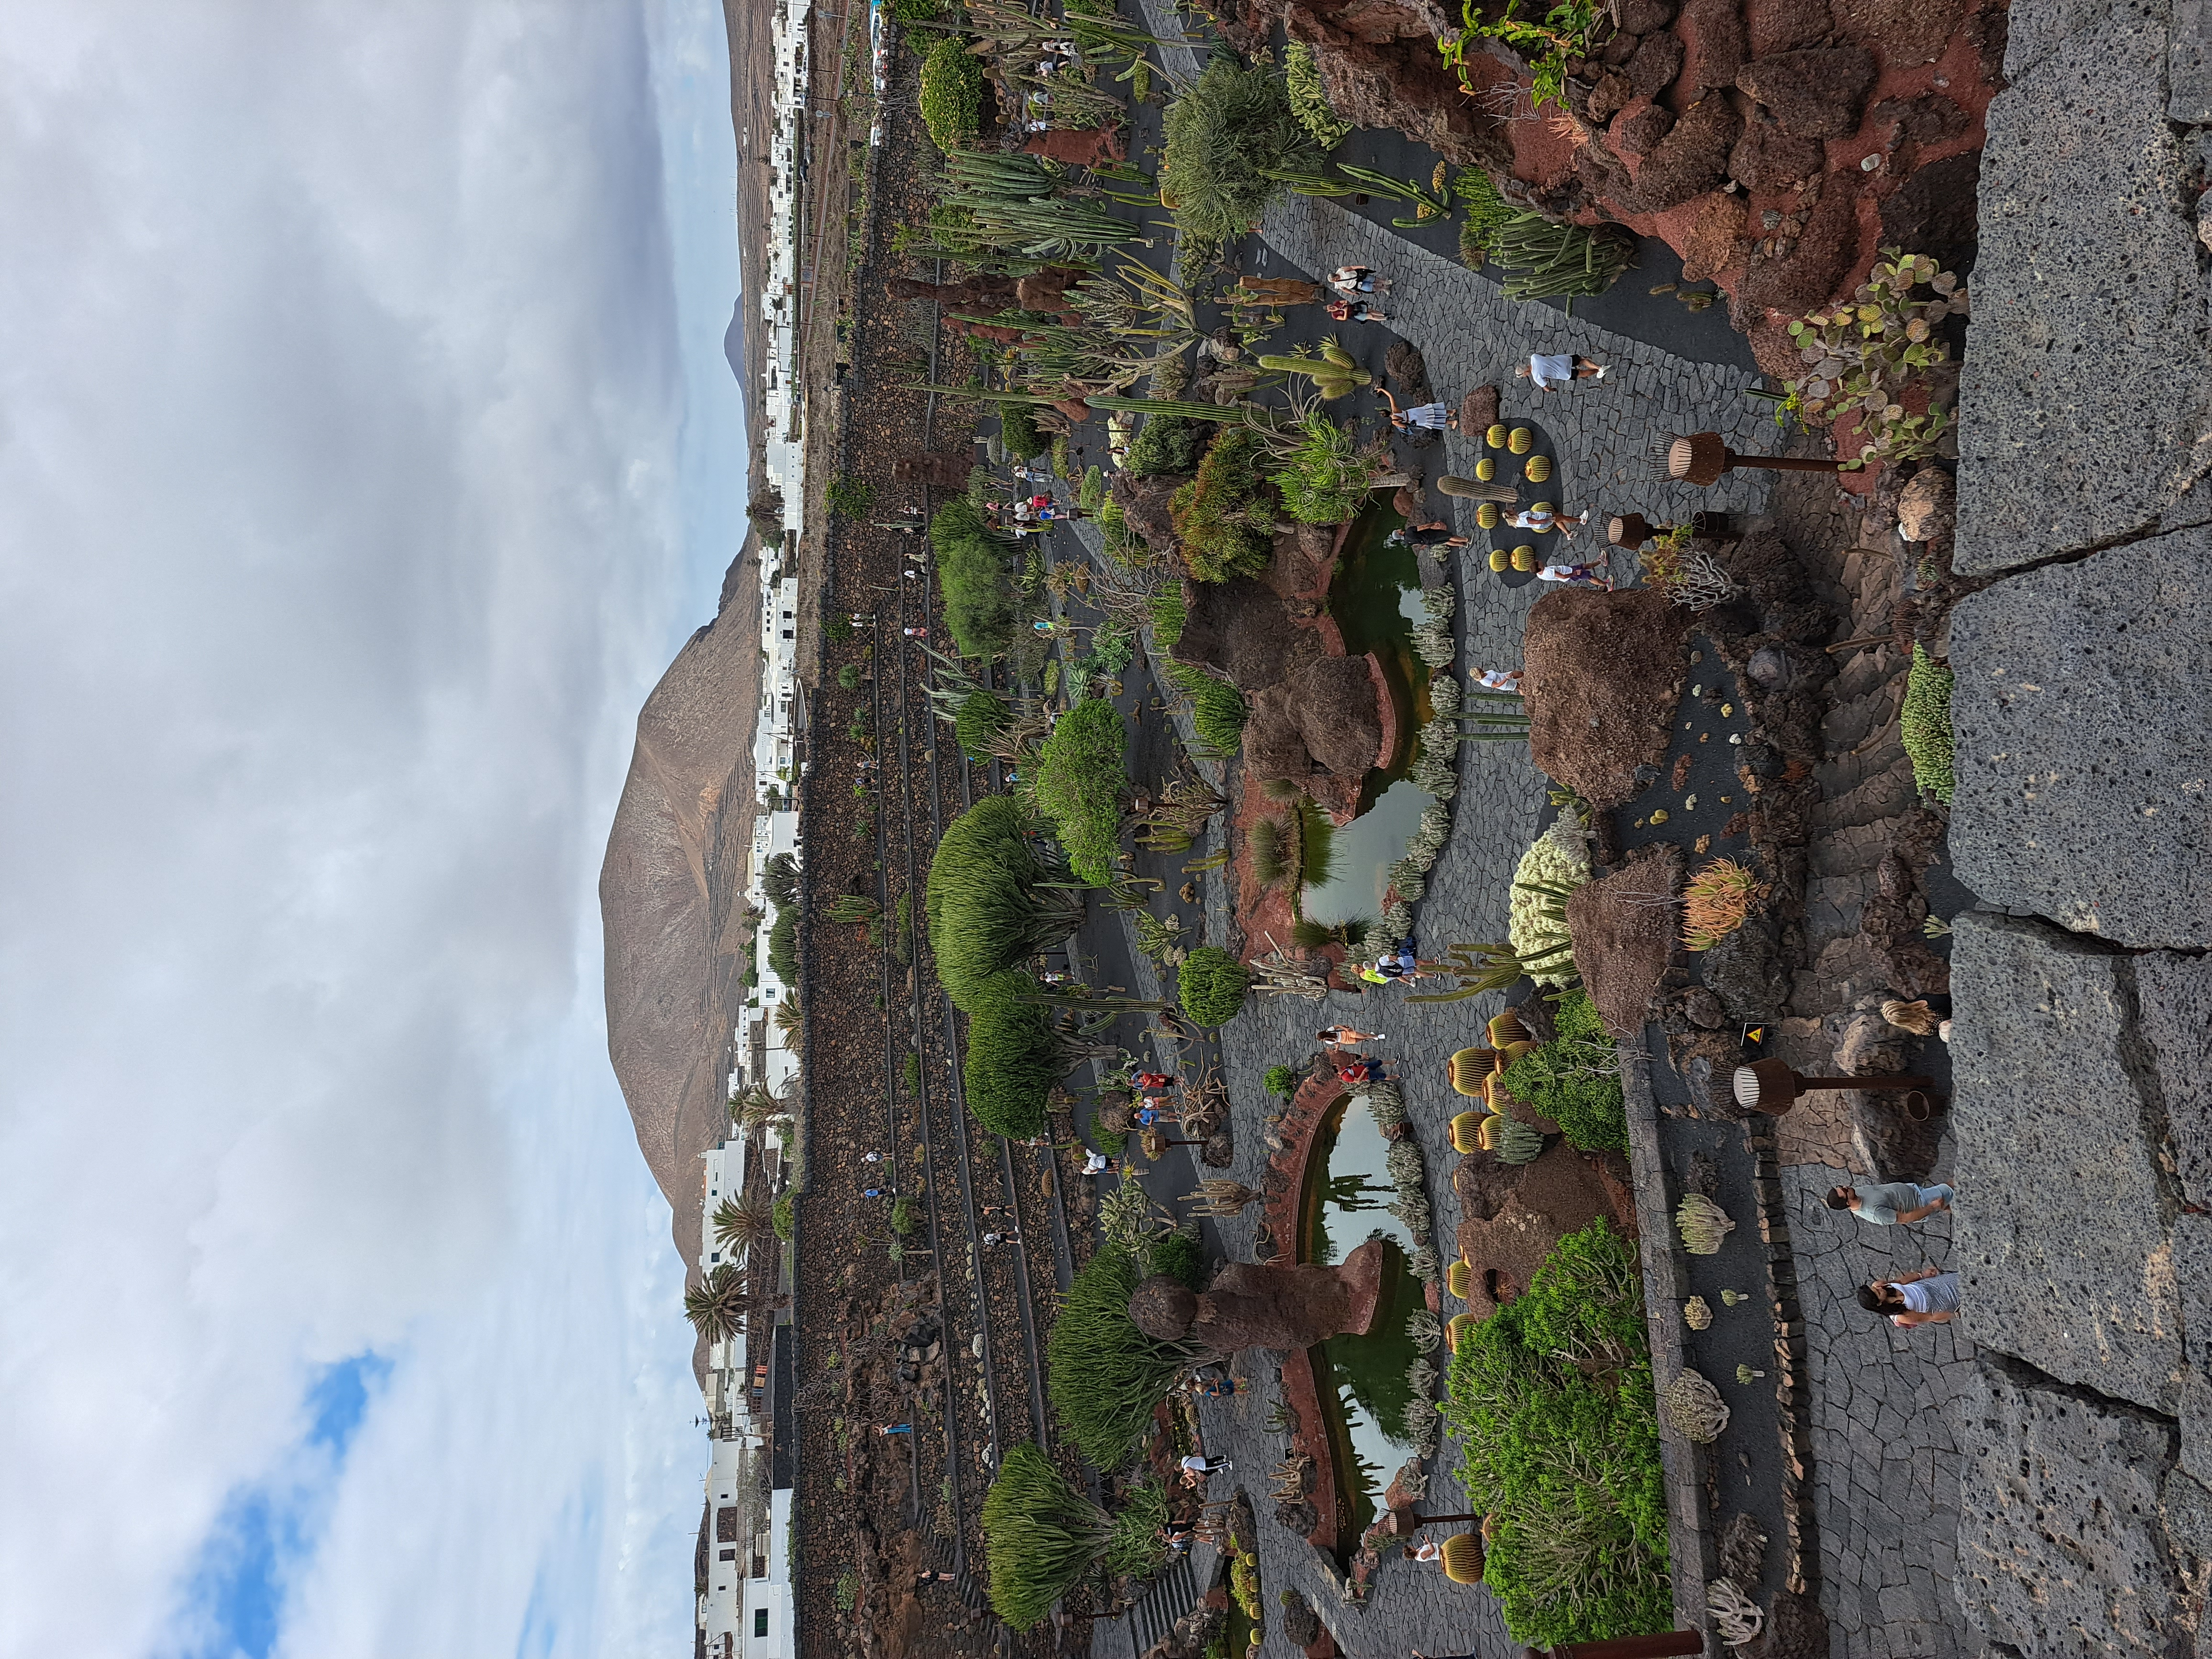
\includegraphics[angle=270, width=0.8\textwidth]{jardin_cactus}
				\label{fig:jardin_cactus}
			\end{column}
			\begin{column}{0.33\textwidth}
				\centering
				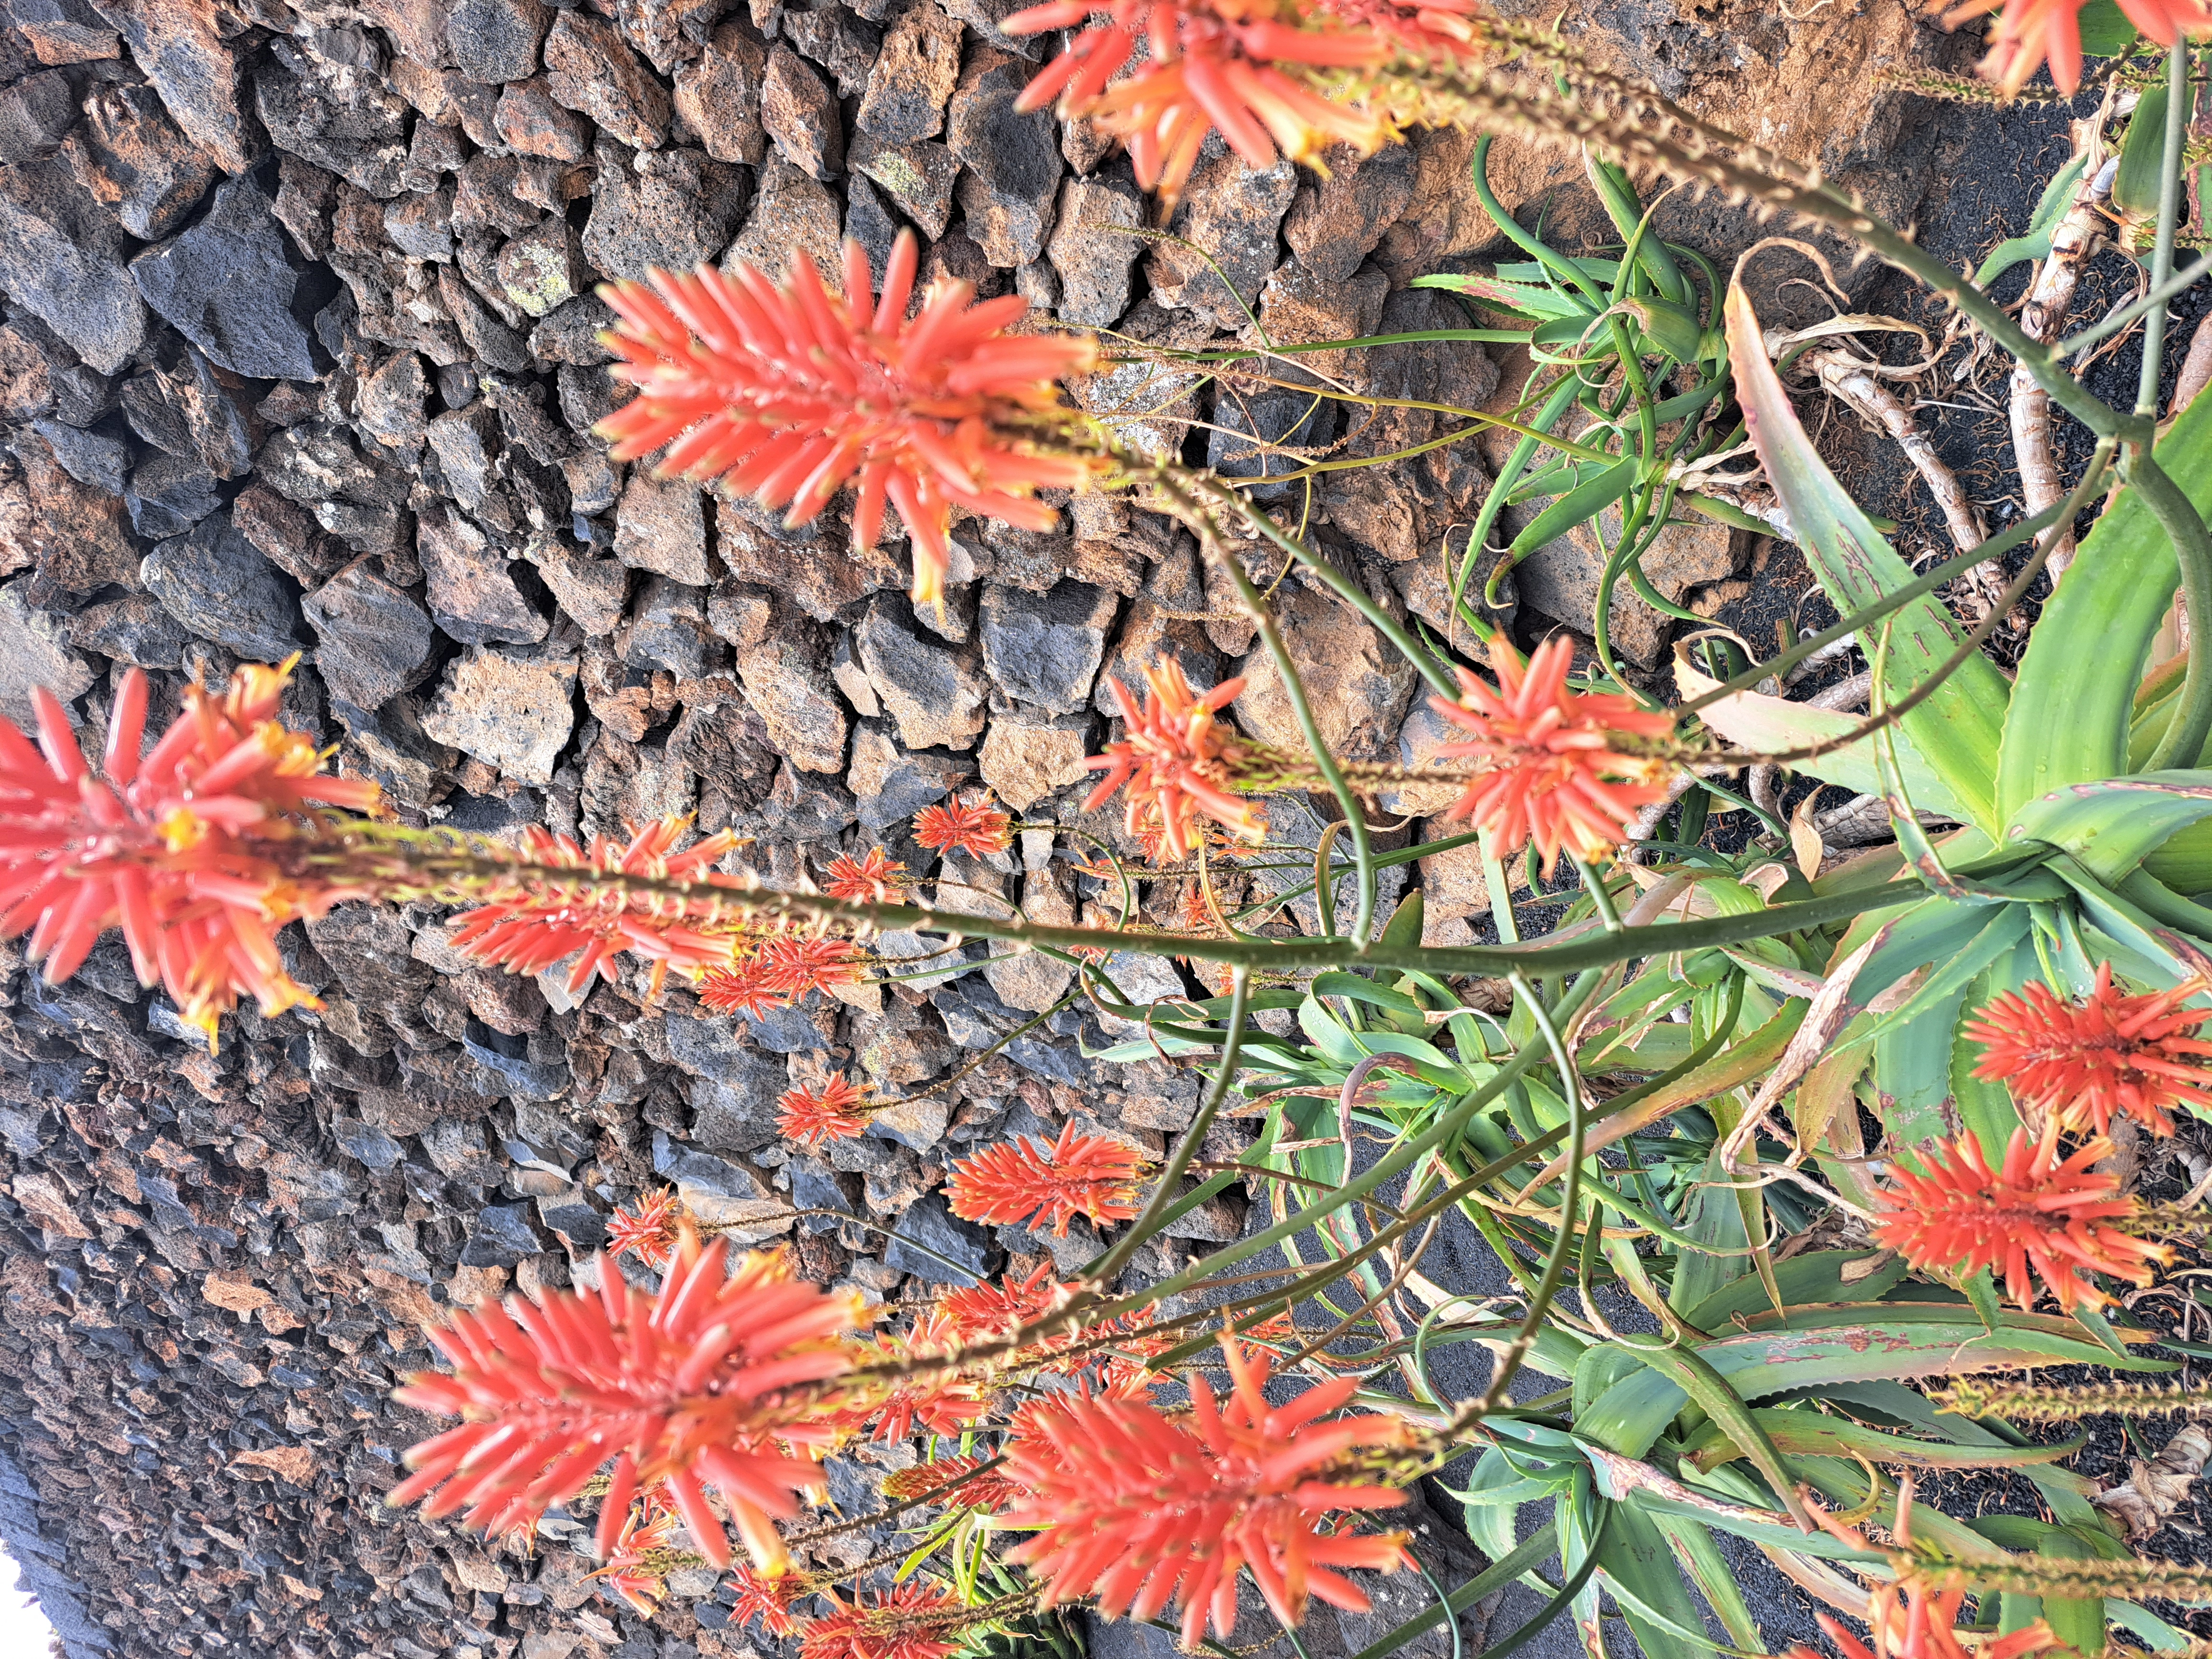
\includegraphics[angle=270, width=0.8\textwidth]{cactus_1}
				\label{fig:cactus_1}
			\end{column}
			\begin{column}{0.33\textwidth}
				\centering
				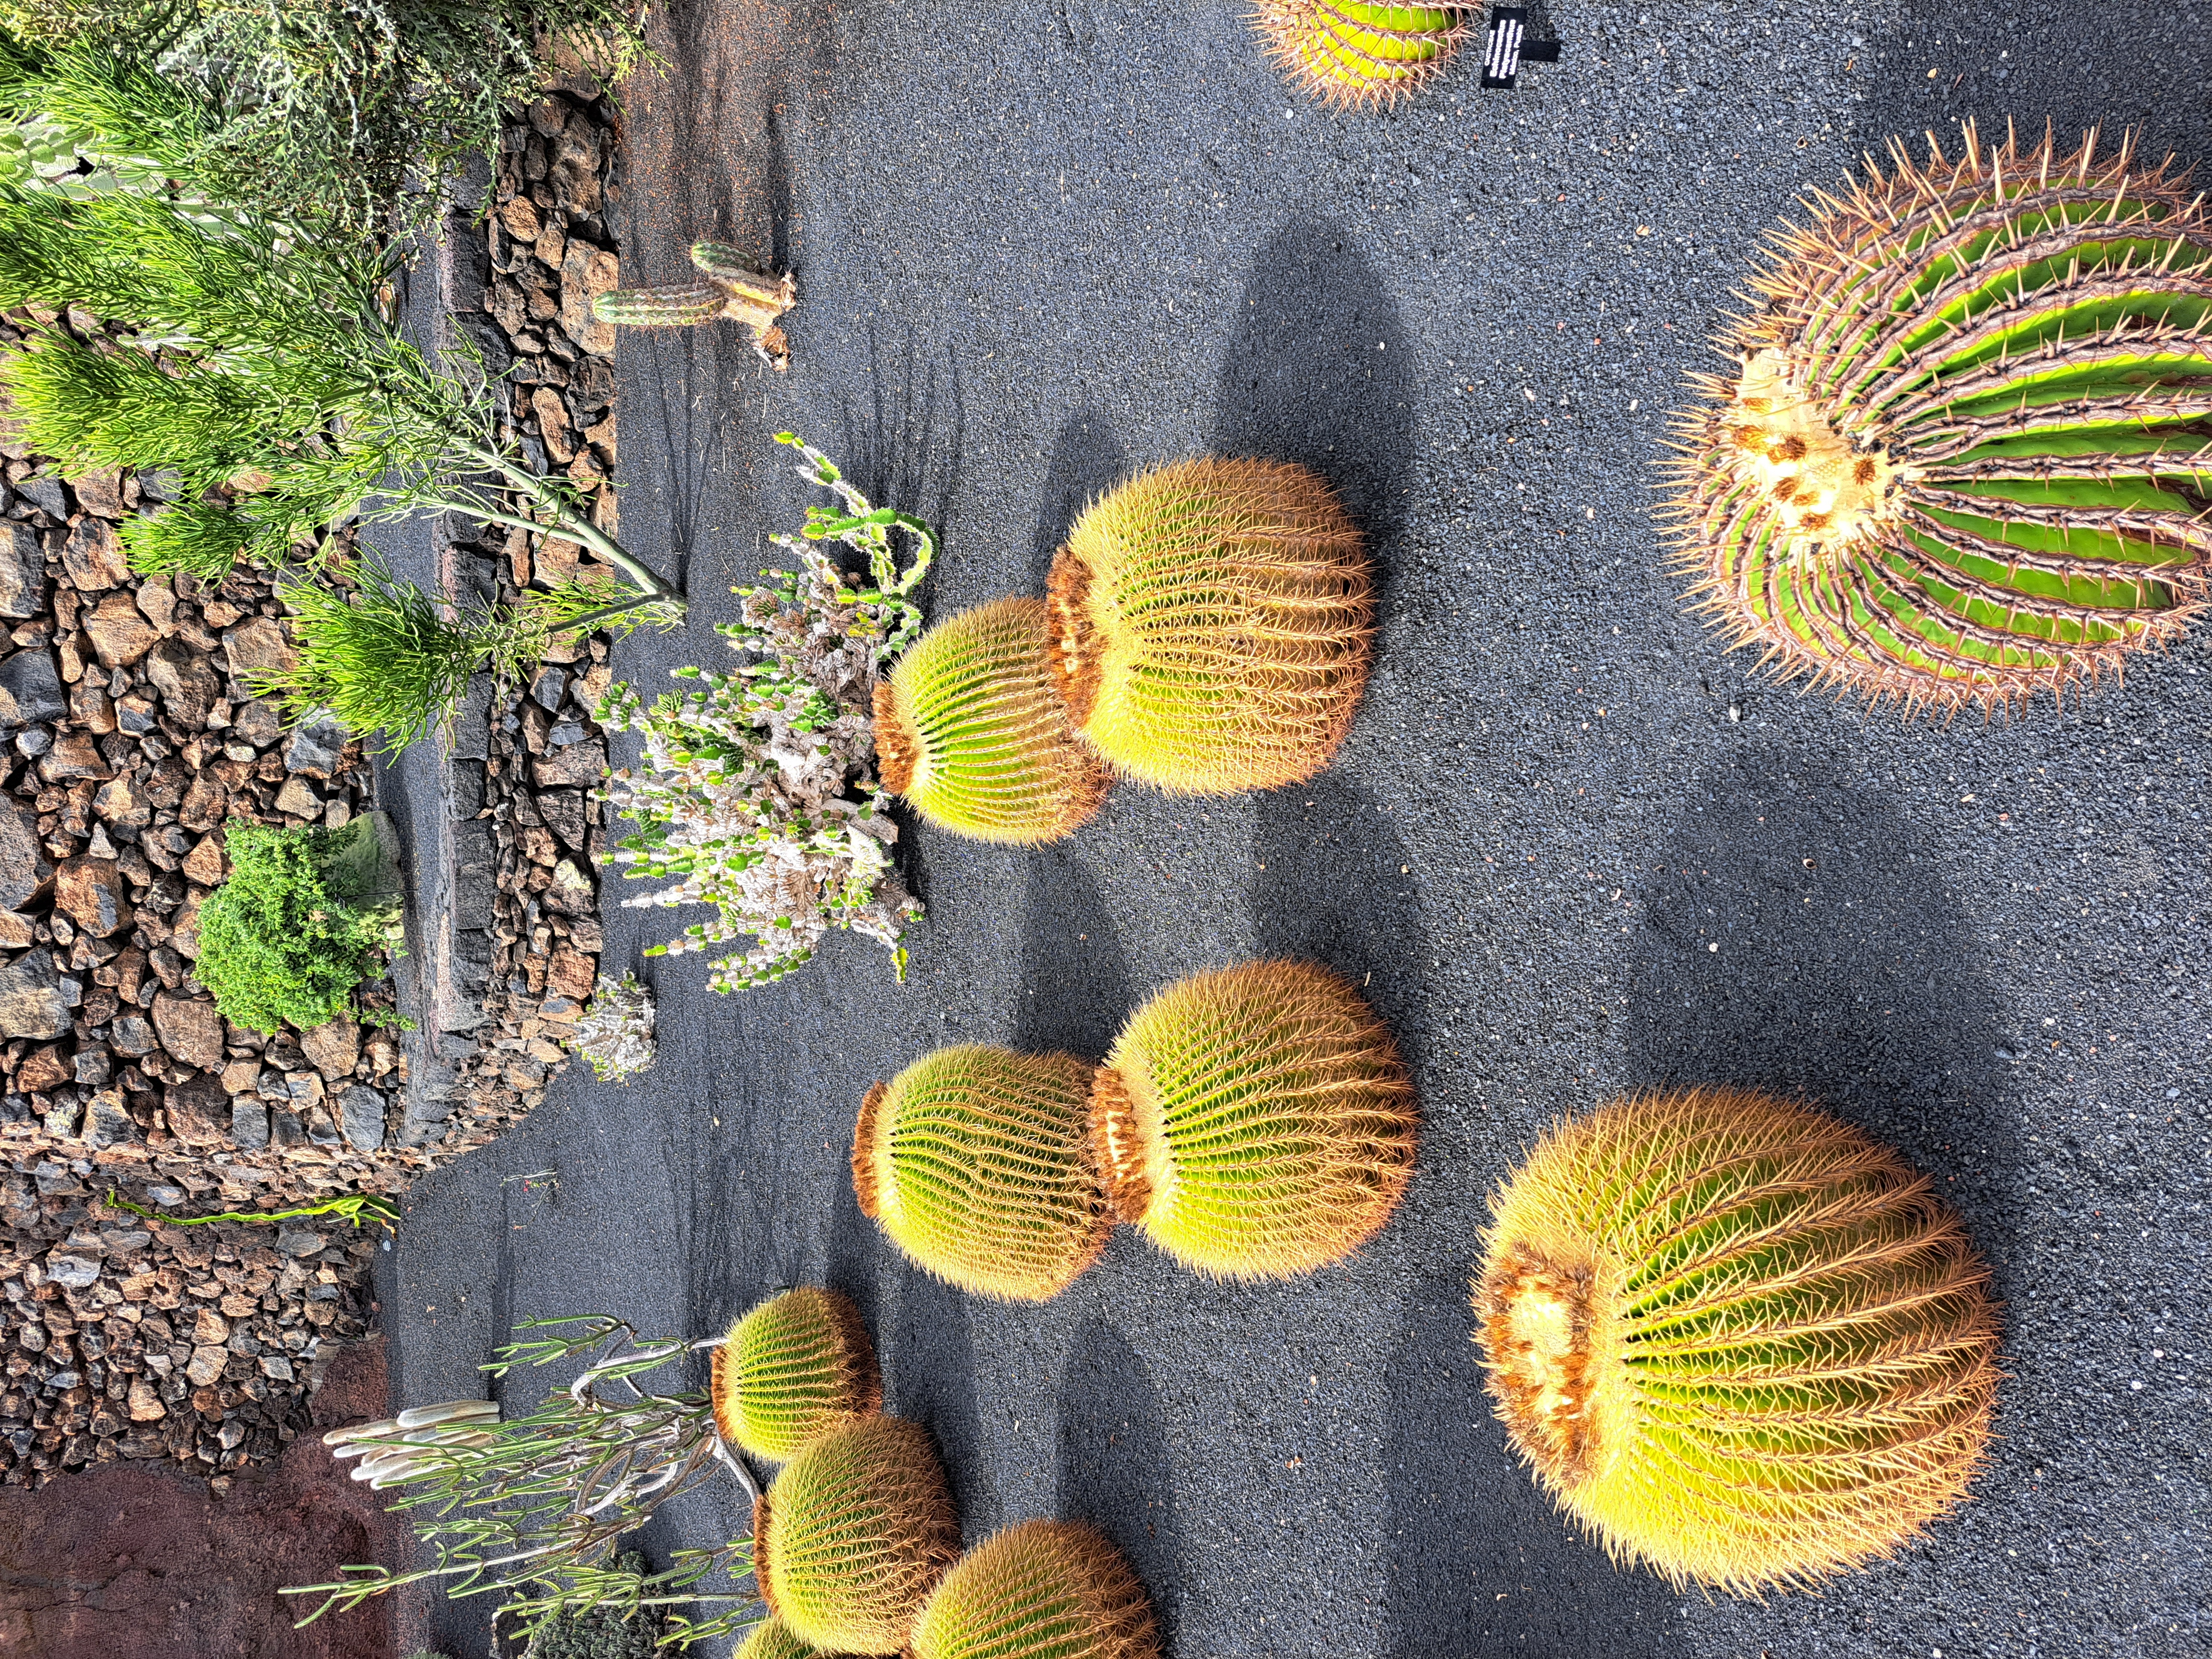
\includegraphics[angle=270, width=0.8\textwidth]{cactus_2}
				\label{fig:cactus_2}
			\end{column}
		\end{columns}
		
	\end{frame}
	
	\begin{frame}
		\frametitle{Cueva de los Verdes}
		Un impresionante túnel volcánico formado por la erupción del Volcán 'La Corona'.
		
		\begin{block}{Un secreto bien guardado}
			Antiguamente servía como refugio contra los piratas. Hoy, es una maravilla natural accesible al público.
		\end{block}
		
		\begin{columns}[c]
			\begin{column}{0.5\textwidth}
				\centering
				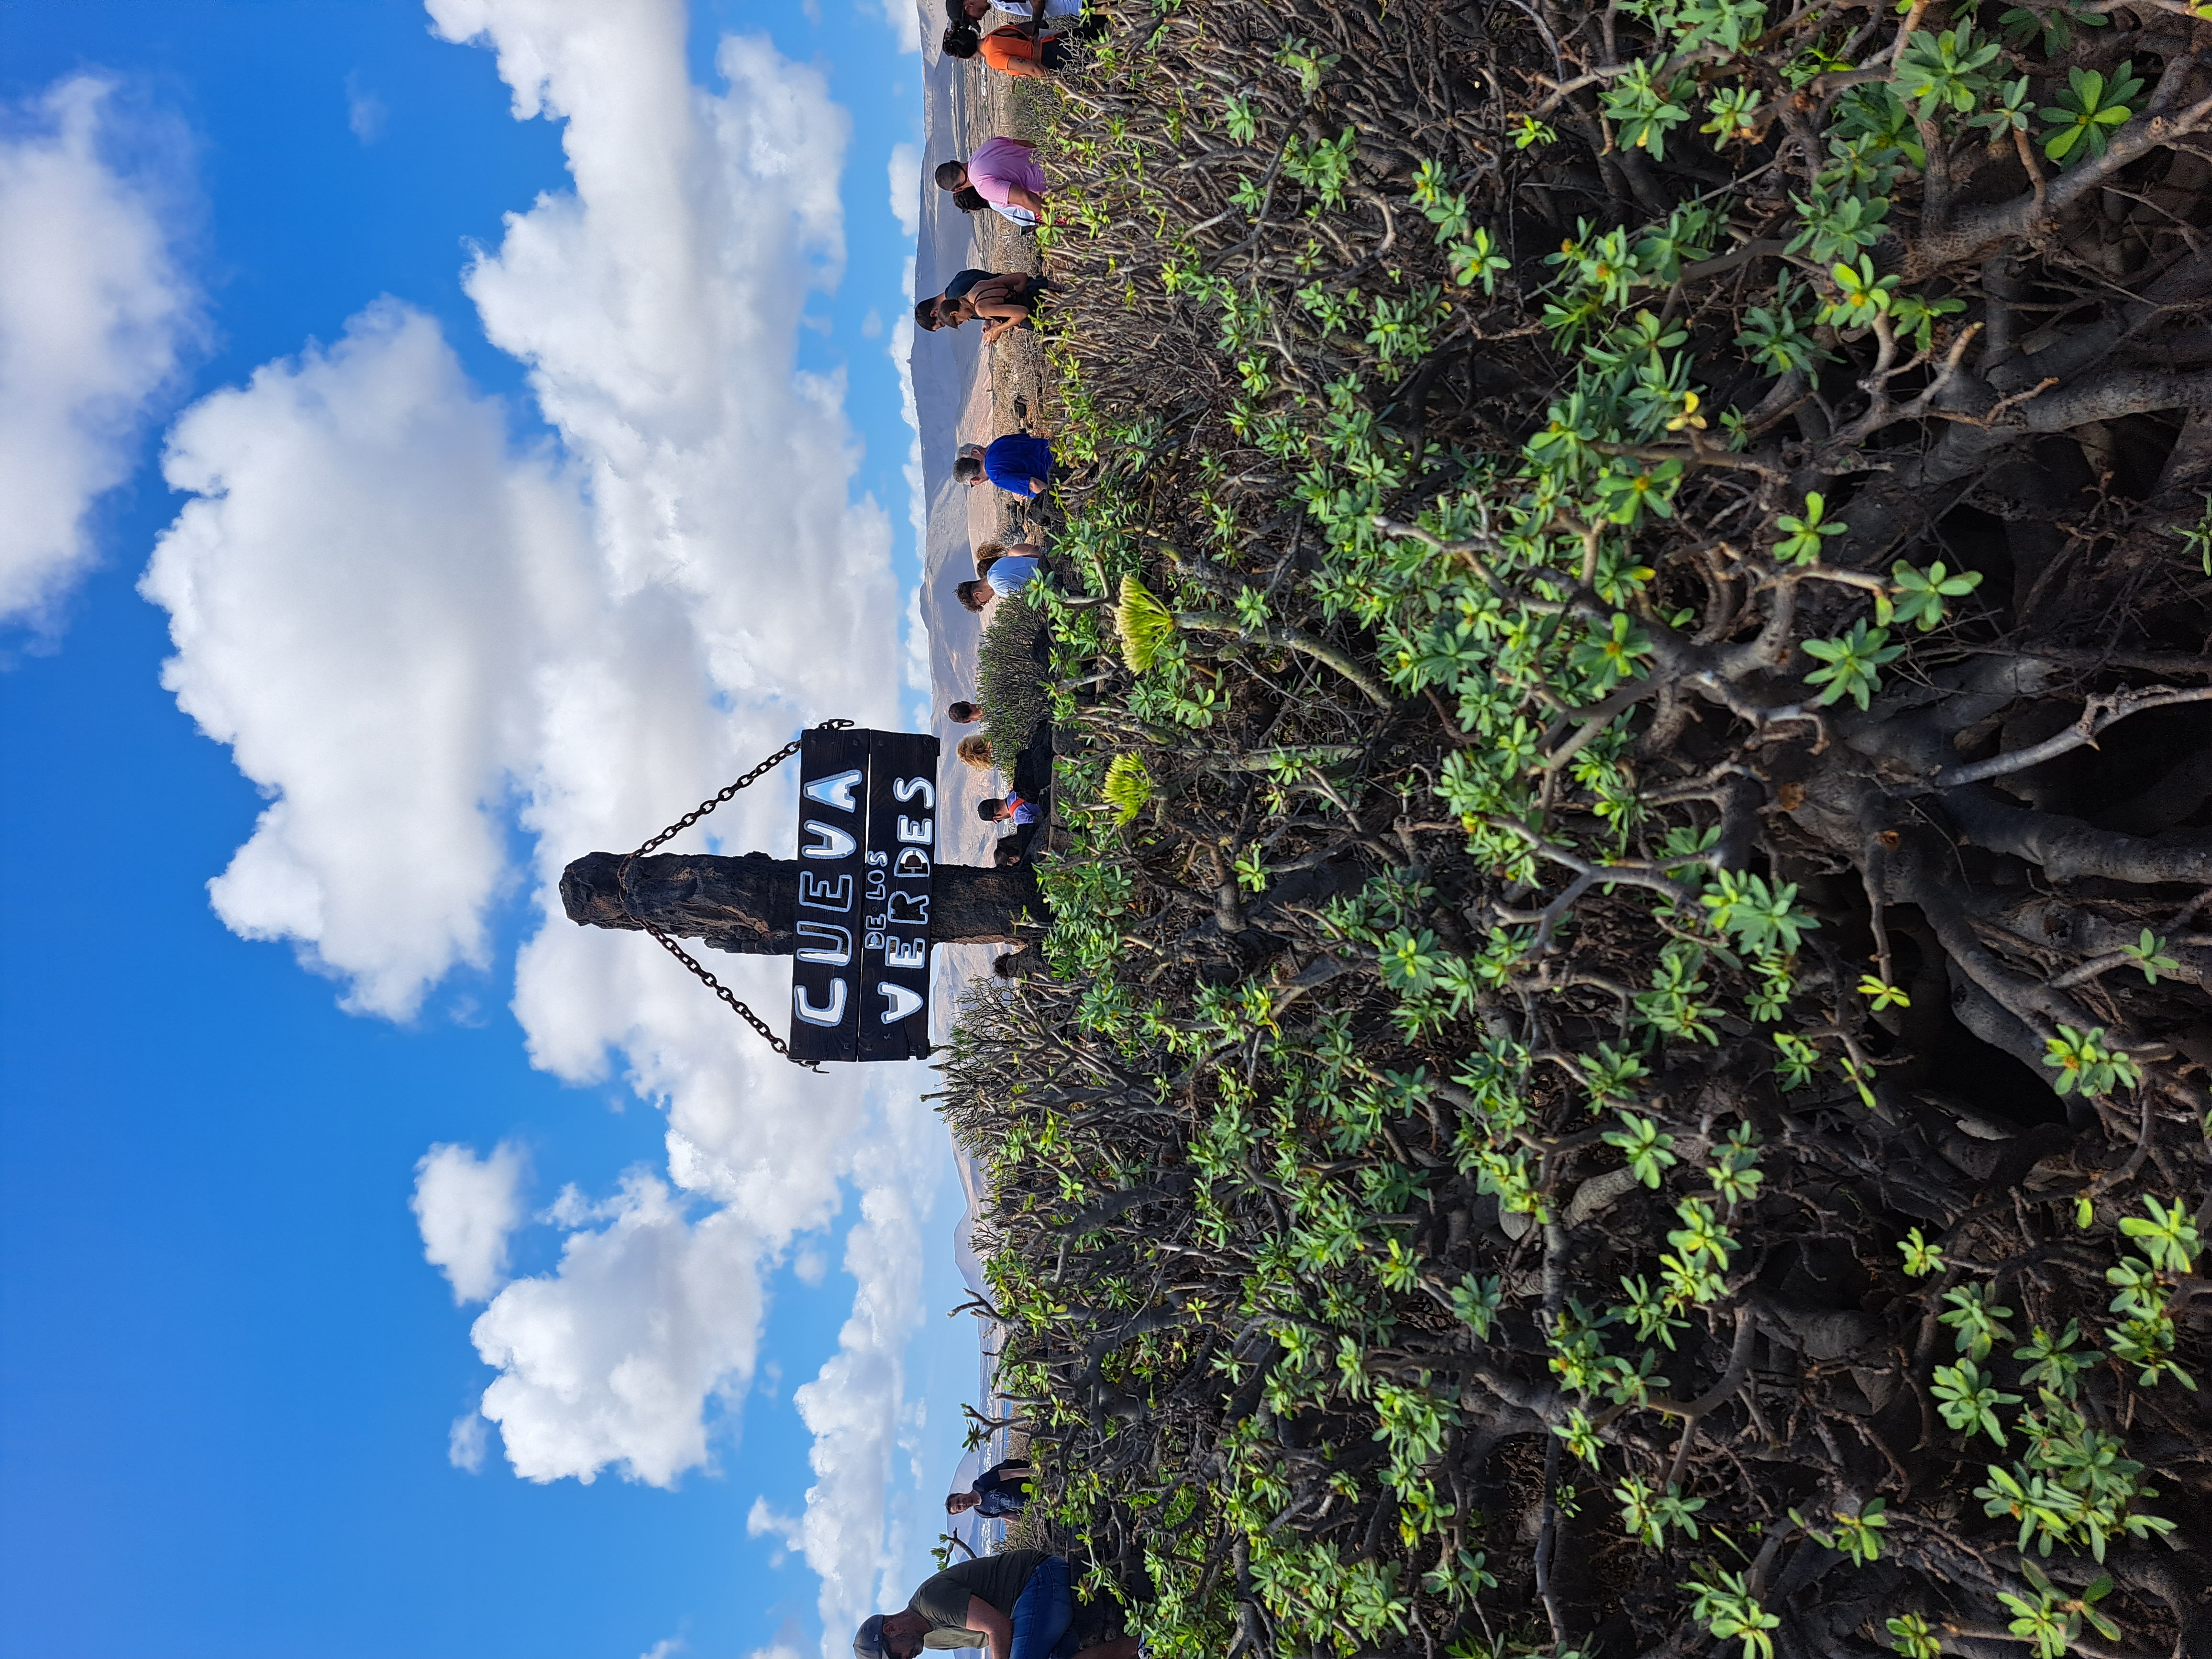
\includegraphics[angle=270, width=0.6\textwidth]{cartel_verdes}
				\label{fig:cartel_verdes}
			\end{column}
			\begin{column}{0.5\textwidth}
				\centering
				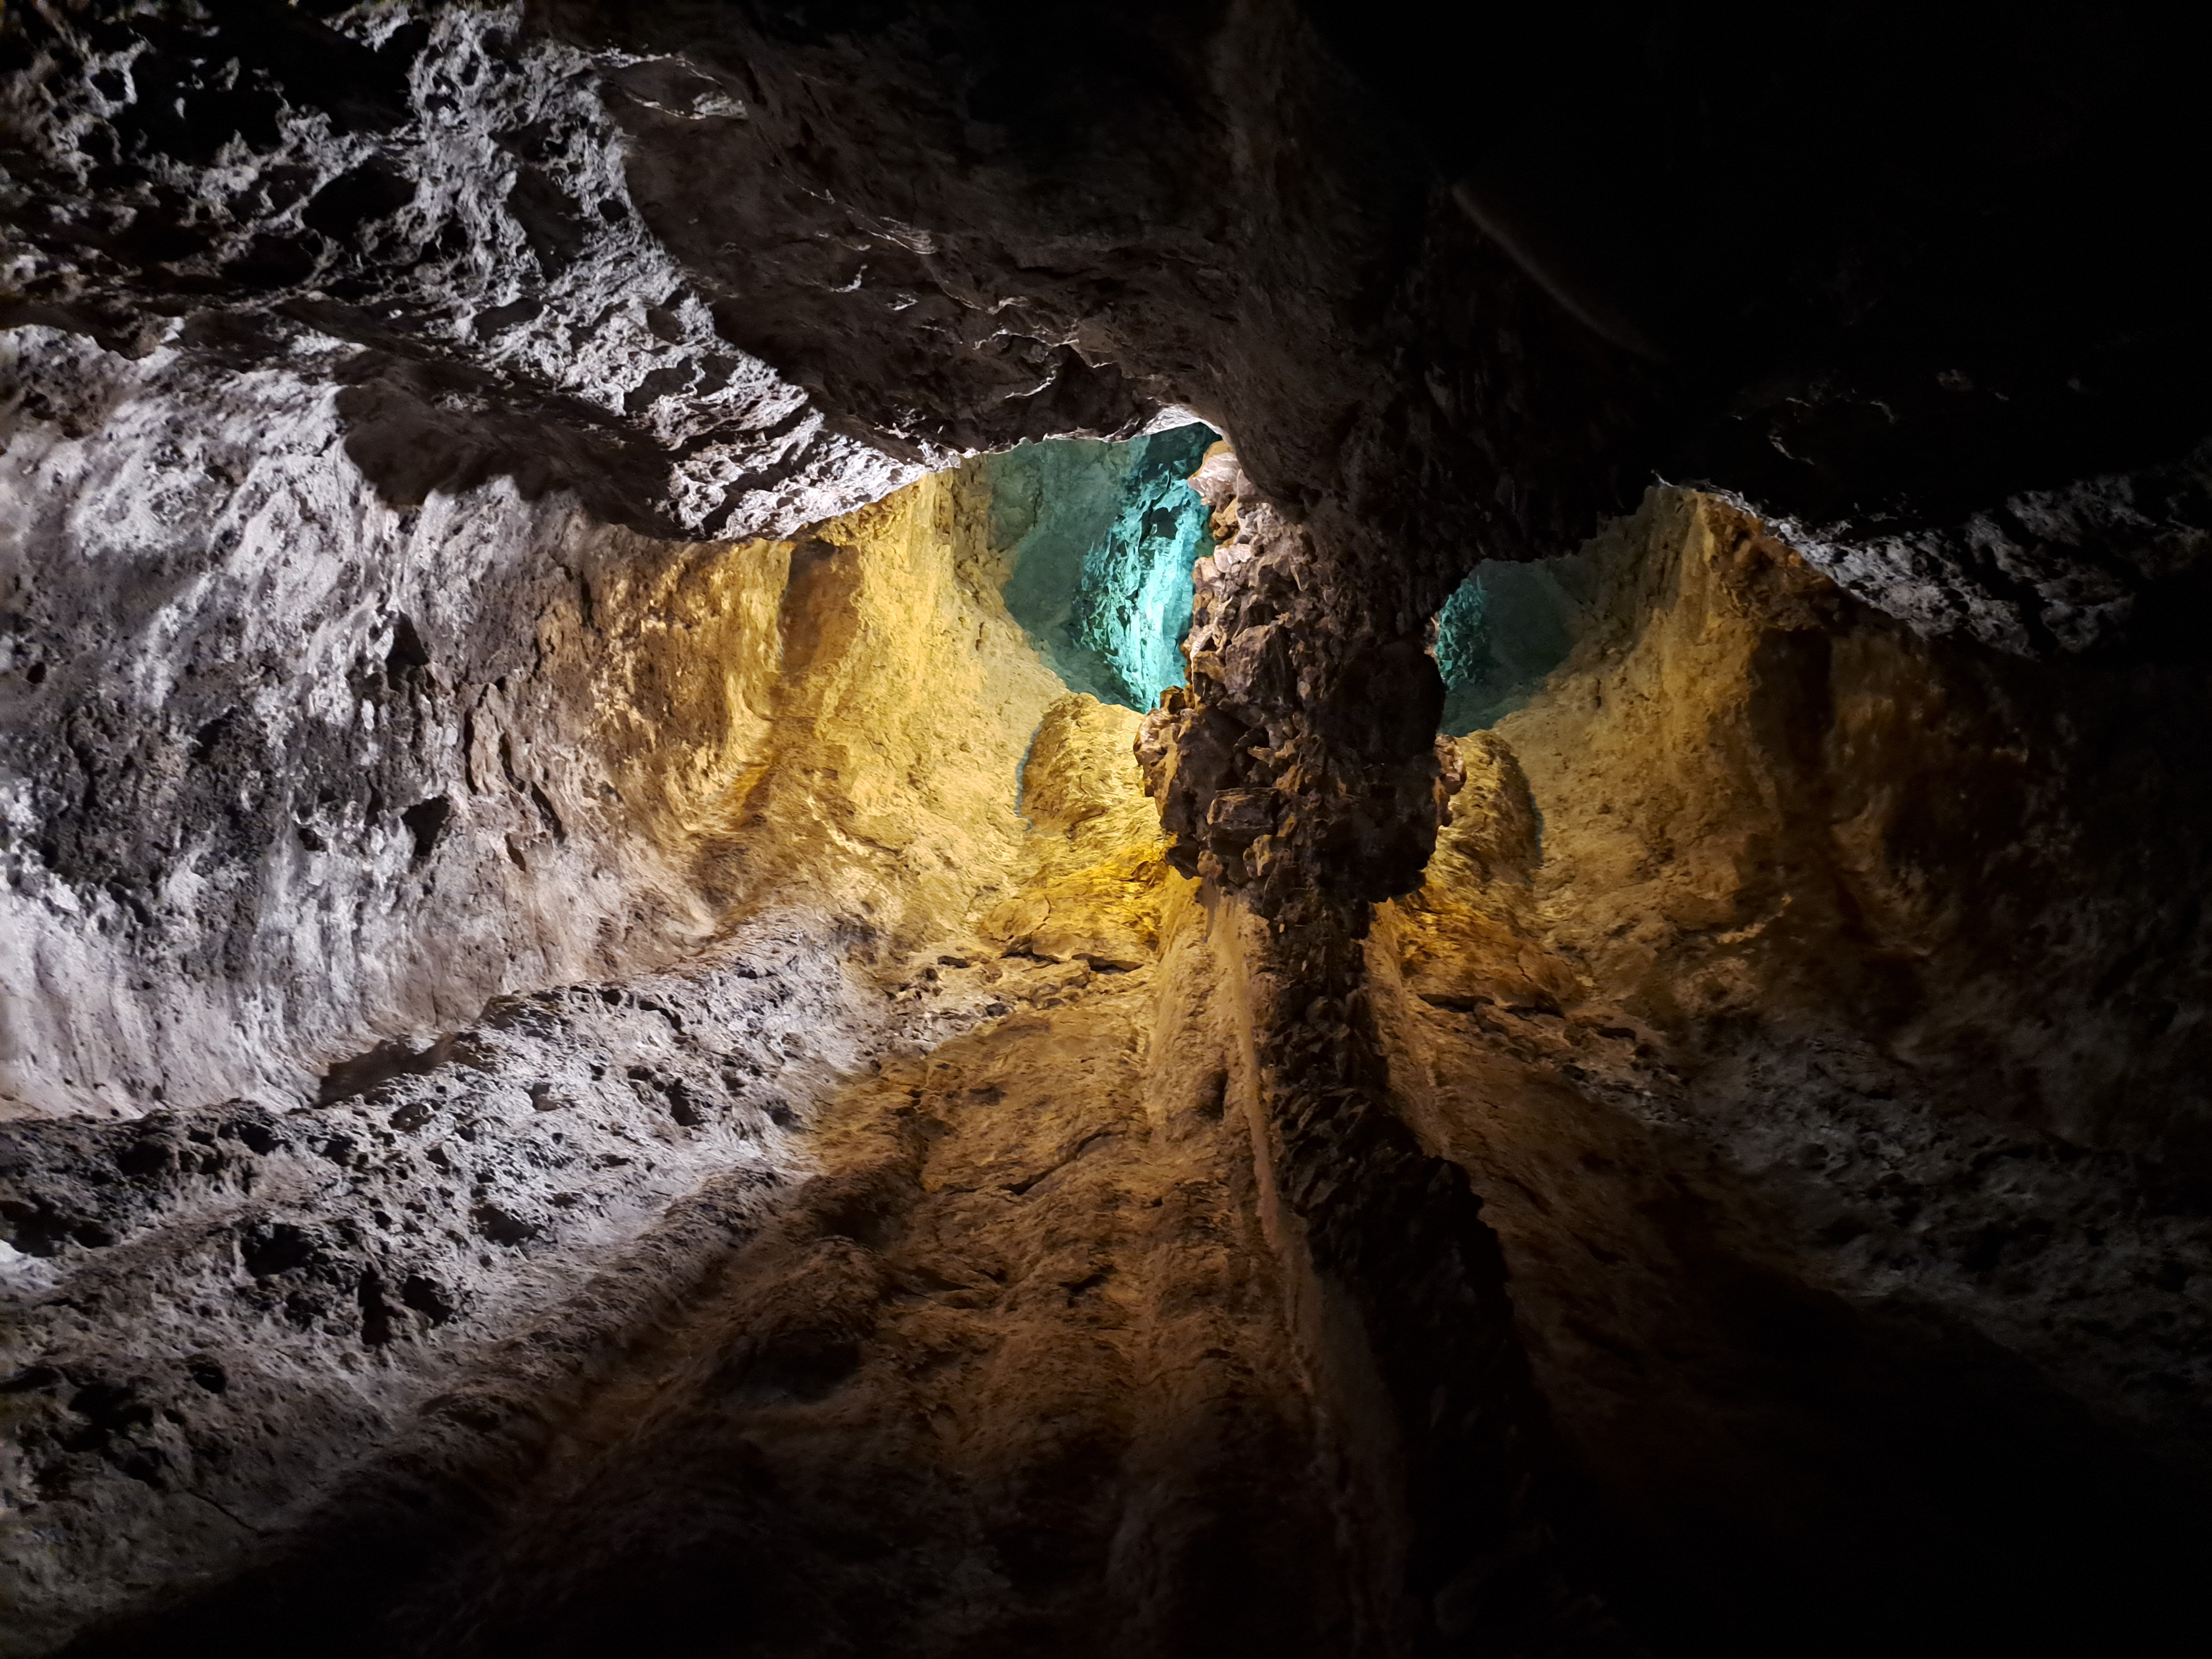
\includegraphics[angle=270, width=0.6\textwidth]{cueva_verdes}
				\label{fig:cueva_verdes}
			\end{column}
		\end{columns}
	\end{frame}
	
	
	
	
	\begin{frame}
		
		\section{Restaurantes Recomendados}
		\frametitle{Restaurantes Recomendados}
		
		\begin{columns}[c]
			\begin{column}{0.5\textwidth}
				\begin{itemize}
					\item \textbf{BAR STRAVA} (Arrecife): Tapas y cocina creativa en un ambiente urbano.
					\item \textbf{EL RECOBECO DE NARA} (Teguise): Cocina tradicional canaria con toques modernos.
					
				\end{itemize}
				\centering
				\includegraphics[width=1\textwidth]{papas}
				\label{fig:papas}
			\end{column}
			\begin{column}{0.5\textwidth}
				\begin{itemize}
					\item \textbf{CAFÉ ANTIGUA ESCUELA} (Yaiza): Cafetería con encanto e historia local.
					\item \textbf{LA CASA DE LA PLAYA} (Arrieta): Cocina con vistas al mar, mariscos frescos.
					
				\end{itemize}
				\centering
				\includegraphics[angle=270, width=0.45\textwidth]{casa}
				\label{fig:casa}
			\end{column}
		\end{columns}
		
		
	\end{frame}
	
	
	
	
	\begin{frame}
		\section{Un día en Lanzarote}
		\frametitle{Un día en Lanzarote}
		
		\begin{block}{\onslide<1->{\textbf{Mañana}}}
			\onslide<1->{Comienza tu aventura en el Parque Nacional de Timanfaya.}
		\end{block}
		
		\begin{alertblock}{\onslide<2->{\textbf{Mediodía}}}
			\onslide<2->{Saborea la gastronomía local en \textit{Café Bar la Escuela}, a solo 6 minutos en coche.}
		\end{alertblock}
		
		\begin{exampleblock}{\onslide<3->{\textbf{Tarde}}}
			\onslide<3->{Visita el Jardín de Cactus y disfruta de su belleza natural.}
		\end{exampleblock}
		
		\only<4>{\vspace{0.3cm}
			\textbf{Consejo final:} Alquila un coche para disfrutar la isla a tu ritmo.}
	\end{frame}
	
	
	
	
	
	\begin{frame}
		\section{Datos curiosos de Lanzarote}
		\frametitle{Datos curiosos de Lanzarote}
		
		\begin{columns}
			\begin{column}{0.5\textwidth}
				\begin{alertblock}{Cultura y Arte}
					\textbf{César Manrique}, artista y arquitecto lanzaroteño, transformó la isla integrando el arte con la naturaleza. \\
					Sus creaciones como Jameos del Agua y el Mirador del Río son imperdibles.
				\end{alertblock}
			\end{column}
			\begin{column}{0.5\textwidth}
				\begin{block}{Naturaleza volcánica}
					Lanzarote es Reserva de la Biosfera por la UNESCO. Cuenta con \textbf{más de 300 conos volcánicos} y paisajes lunares \textbf{únicos en Europa}.
				\end{block}
			\end{column}
		\end{columns}
	\end{frame}
	

	\begin{frame}
		\section{Vida marina en Lanzarote}
		\frametitle{Vida marina en Lanzarote}
		
		La diversidad y cantidad de cetáceos que habitan las aguas que rodean las islas de Lanzarote y Fuerteventura las han convertido en el foco de una campaña impulsada por WWF para crear un \textbf{SANTUARIO DE CETÁCEOS}. El objetivo es garantizar la preservación de la zona para la conservación de las especies y su hábitat.

		\pause
		
		\begin{block}{¡Una de las islas con mayor diversidad!}
			Se tienen registros de al menos 29 especies de cetáceos, entre delfines, zifios, calderones, cachalotes…, que viven o pasan en su migración por las aguas que rodean estas islas.
		\end{block}
		
	\end{frame}
	
	\begin{frame}
		\frametitle{Vida marina en Lanzarote}
		
		\begin{alertblock}{¿Te apetece bucear?}
			Lanzarote tiene algunos de los mejores fondos marinos de Europa, la formación rocosa y volcánica de las islas Canarias hacen que el mundo submarino de la isla sea increíble. La visibilidad que alcanza unos 40 metros, las temperaturas subtropicales y la abundancia y variedad de especies marinas te asombrarán.
		\end{alertblock}
		
	\end{frame}


\begin{frame}
	\section{Puntos de buceo}
	\frametitle{All you need is buceo}
	
	 La isla se divide en 4 zonas de buceo: 
	
	\begin{columns}
		\begin{column}{0.48\textwidth}
			\begin{itemize}
				\item \onslide<1->{\textbf{Playa Blanca}: es una de las zonas más tranquilas para el buceo, no se superan profundidades de 18 metros y está protegida de los vientos alisios del norte.}
			\end{itemize}
		\end{column}
		
		\begin{column}{0.48\textwidth}
			\begin{itemize}
				\item \onslide<2->{\textbf{Puerto del Carmen}: en el centro este de la isla, bajo Arrecife, es probablemente la zona más concurrida de la isla para bucear. Las inmersiones se realizan a lo largo de su veril, una impresionante pared que empieza en 15 metros y desciende hasta los 40.}
			\end{itemize}
		\end{column}
	\end{columns}
	
	
\end{frame}

\begin{frame}
	\frametitle{All you need is buceo}
	
	La isla se divide en 4 zonas de buceo: 
	
	\begin{columns}
		\begin{column}{0.48\textwidth}
			\begin{itemize}
				\item \onslide<1->{\textbf{Mala}: se encuentra al noroeste de la isla, junto a los pueblos de Arrieta y Charco del Palo. Es una de nuestros sitios de buceo preferidos por sus paisajes submarinos. Impresionantes pendientes de arena blanca que se pierden en el azul cortadas perpendicularmente por lenguas volcánicas que descienden hacia las profundidades.}
			\end{itemize}
		\end{column}
	
		
		\begin{column}{0.48\textwidth}
			\begin{itemize}
				\item \onslide<2->{\textbf{La Graciosa}: es un espacio natural protegido y constituye la reserva marina más grande de Europa.}
			\end{itemize}
		\end{column}
	\end{columns}
	
	
\end{frame}

\end{document}
